% ---------------------------------------------------------------------------
% Demonstration deck for beamer2pptx.
%
% Convert it with:
%   python beamer2pptx.py examples/demo/demo.tex -o out/demo.pptx
%
% It is a deliberately ordinary Beamer talk: nothing here is written for the
% converter's benefit.
% ---------------------------------------------------------------------------
\documentclass[aspectratio=43]{beamer}
\usetheme{Madrid}

\usepackage{amsmath, amssymb}
\usepackage{booktabs}
\usepackage{multirow}
\usepackage{graphicx}
\usepackage{tikz}
\usepackage{pgfplots}
\pgfplotsset{compat=1.18}
\usetikzlibrary{arrows.meta, positioning}

\graphicspath{{figures/}}

% User macros: expanded before parsing, so they work in text and in maths.
\newcommand{\R}{\mathbb{R}}
\newcommand{\vect}[1]{\mathbf{#1}}
\newcommand{\unit}[1]{\,\mathrm{#1}}
\DeclareMathOperator*{\argmin}{arg\,min}

\title{Model-Based Estimation of Plantar Pressure}
\subtitle{A demonstration of Beamer to PowerPoint conversion}
\author{Abolfazl Mohebbi}
\institute{Polytechnique Montr\'eal}
\date{\today}

\begin{document}

\begin{frame}
  \titlepage
\end{frame}

% ---------------------------------------------------------------------------
\section{Motivation}

\begin{frame}{Why estimate what we can measure?}
  \begin{itemize}
    \item Instrumented insoles are \alert{expensive} and drift over long trials.
    \item A model lets us infer pressure from \textbf{kinematics alone},
          recorded with \textcolor{blue}{ordinary motion capture}.
    \item Three requirements drive the design:
      \begin{itemize}
        \item accuracy within clinical tolerance, $e < 5\%$;
        \item real-time evaluation at $100\unit{Hz}$;
        \item subject-specific calibration from one walking trial.
          \begin{itemize}
            \item[$\star$] no force plate needed after calibration
          \end{itemize}
      \end{itemize}
    \item Data and code: \url{https://example.org/plantar-dataset}
  \end{itemize}
\end{frame}

\begin{frame}{Approach at a glance}
  \begin{block}{Working hypothesis}
    Ground reaction force distributes across the foot as a low-rank
    combination of a small number of pressure modes.
  \end{block}

  \begin{itemize}
    \item Learn the modes once, offline.
    \pause
    \item Fit per-subject weights from a single trial.
    \item<3-> Evaluate the model online, one matrix product per frame.
  \end{itemize}

  \begin{alertblock}{Caveat}
    The low-rank assumption degrades for pathological gait, where
    $\argmin_{\vect{w}} \|\vect{p} - \Phi\vect{w}\|$ is poorly conditioned.
  \end{alertblock}
\end{frame}

% ---------------------------------------------------------------------------
\section{Formulation}

\begin{frame}{The estimator}
  Measured pressure $\vect{p} \in \R^{n}$ is approximated by $r \ll n$ modes,
  so that $\vect{p} \approx \Phi \vect{w}$ with $\Phi \in \R^{n \times r}$.

  \[
    \vect{w}^\star = \argmin_{\vect{w} \in \R^{r}}
      \; \|\vect{p} - \Phi\vect{w}\|_2^2 + \lambda \|\vect{w}\|_2^2
  \]

  The regularised normal equations give a closed form, and the residual
  follows immediately:
  \begin{align}
    \vect{w}^\star &= (\Phi^\top \Phi + \lambda I)^{-1} \Phi^\top \vect{p} \\
    \vect{r}       &= \vect{p} - \Phi \vect{w}^\star
  \end{align}

  For two modes the projection matrix is simply
  \[
    \Phi^\top \Phi = \begin{bmatrix}
      \phi_{11} & \phi_{12} \\
      \phi_{21} & \phi_{22}
    \end{bmatrix} .
  \]
\end{frame}

\begin{frame}{Well-posedness}
  \begin{theorem}[Unique minimiser]
    For every $\lambda > 0$ the objective is strictly convex, so
    $\vect{w}^\star$ exists and is unique.
  \end{theorem}

  \begin{description}
    \item[Input] kinematic frame $\vect{q} \in \R^{23}$
    \item[Output] pressure field $\hat{\vect{p}} \in \R^{99}$
    \item[Cost] one $99 \times 6$ product per frame
  \end{description}
\end{frame}

% ---------------------------------------------------------------------------
\section{Results}

\begin{frame}{Accuracy against the instrumented insole}
  \begin{table}
    \centering
    \begin{tabular}{llrrr}
      \toprule
      \multirow{2}{*}{Cohort} & \multirow{2}{*}{Model} &
        \multicolumn{2}{c}{Error (\%)} & \multirow{2}{*}{Rate (Hz)} \\
      \cmidrule(lr){3-4}
       &  & Peak & RMS &  \\
      \midrule
      \multirow{2}{*}{Healthy}  & Baseline      & 11.4 & 6.2 & 42 \\
                                & \textbf{Ours} &  4.1 & 2.3 & 118 \\
      \midrule
      \multirow{2}{*}{Post-op}  & Baseline      & 18.9 & 9.7 & 42 \\
                                & \textbf{Ours} &  6.8 & 3.9 & 116 \\
      \midrule
      \multicolumn{4}{l}{Mean improvement over baseline} & $2.7\times$ \\
      \bottomrule
    \end{tabular}
    \caption{Six modes, leave-one-subject-out validation ($n = 24$).}
  \end{table}
\end{frame}

\begin{frame}{Pipeline and convergence}
  \begin{columns}
    \begin{column}{0.52\textwidth}
      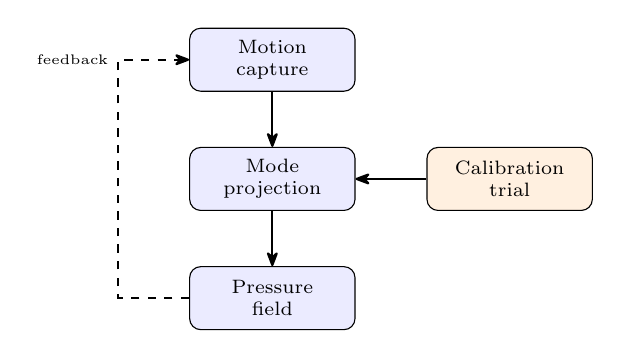
\begin{tikzpicture}[
          node distance = 7mm and 9mm,
          box/.style = {draw, rounded corners, fill=blue!8,
                        minimum width=21mm, minimum height=8mm,
                        align=center, font=\scriptsize},
          >={Stealth[round]}]
        \node[box] (mocap) {Motion\\capture};
        \node[box, below=of mocap] (model) {Mode\\projection};
        \node[box, below=of model] (out)   {Pressure\\field};
        \node[box, right=of model, fill=orange!12] (cal) {Calibration\\trial};
        \draw[->, thick] (mocap) -- (model);
        \draw[->, thick] (model) -- (out);
        \draw[->, thick] (cal)   -- (model);
        \draw[->, thick, dashed] (out.west) -- ++(-9mm,0)
              |- (mocap.west) node[midway, left, font=\tiny] {feedback};
      \end{tikzpicture}
    \end{column}
    \begin{column}{0.44\textwidth}
      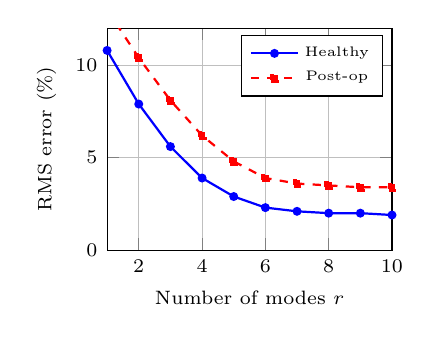
\begin{tikzpicture}
        \begin{axis}[
            width=5.2cm, height=4.4cm,
            xlabel={Number of modes $r$}, ylabel={RMS error (\%)},
            xmin=1, xmax=10, ymin=0, ymax=12,
            grid=major, tick label style={font=\scriptsize},
            label style={font=\scriptsize},
            legend style={font=\tiny, at={(0.97,0.97)}, anchor=north east}]
          \addplot[thick, blue, mark=*, mark size=1.2pt]
            coordinates {(1,10.8)(2,7.9)(3,5.6)(4,3.9)(5,2.9)
                         (6,2.3)(7,2.1)(8,2.0)(9,2.0)(10,1.9)};
          \addlegendentry{Healthy}
          \addplot[thick, red, dashed, mark=square*, mark size=1.2pt]
            coordinates {(1,13.0)(2,10.4)(3,8.1)(4,6.2)(5,4.8)
                         (6,3.9)(7,3.6)(8,3.5)(9,3.4)(10,3.4)};
          \addlegendentry{Post-op}
        \end{axis}
      \end{tikzpicture}
    \end{column}
  \end{columns}
\end{frame}

\begin{frame}{Reconstructed pressure field}
  \begin{figure}
    \centering
    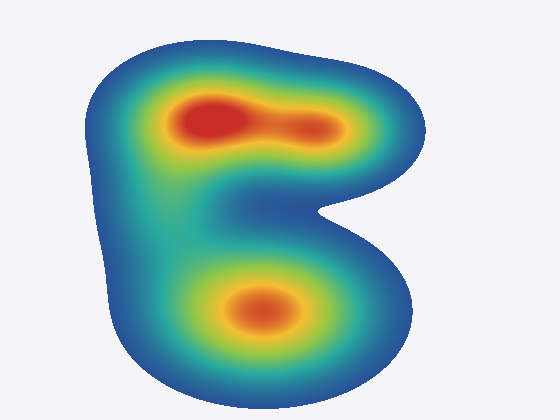
\includegraphics[width=0.52\textwidth]{pressure-map.png}
    \caption{Estimated peak-pressure distribution at mid-stance.}
  \end{figure}
\end{frame}

% ---------------------------------------------------------------------------
\section{Implementation}

\begin{frame}[fragile]{Evaluating the model}
  The online step is a single regularised solve:
  \begin{verbatim}
def estimate(phi, p, lam=1e-3):
    g = phi.T @ phi + lam * np.eye(phi.shape[1])
    w = np.linalg.solve(g, phi.T @ p)   % one solve per frame
    return phi @ w
  \end{verbatim}
  Called once per frame; \verb|phi| is cached after calibration.
  \note{Mention that the solve is 6x6, so cost is negligible.}
\end{frame}

\begin{frame}{Takeaways}
  \begin{itemize}
    \item Six modes reach clinical tolerance on both cohorts.
    \item Runs at $118\unit{Hz}$ on a laptop, well above the $100\unit{Hz}$ target.
    \item Calibration needs one trial, not a force plate per session.
  \end{itemize}
  \begin{block}{Next}
    Extend the mode basis to pathological gait, where the current
    low-rank assumption is weakest.
  \end{block}
\end{frame}

\end{document}
